\section{弱导数}
\label{sec:weakd-weak-derivatives}

绝对值函数$\lvert x\rvert$在原点没有导数，但除了这一点以外，它的导数$\operatorname{sgn}x$处处存在，而且一个点并不承载长度。阶跃函数$\mathbf 1_{(0,\infty)}$也只在原点没有导数，其余各点导数都是零，可它在原点确实有一次变化。逐点导数分不清这两种情形，我们改用积分来描述变化。

\subsection{经典导数的测试恒等式}
\label{sec:weakd-test-identity}

先在有限维看导数怎样“转移”。对数列定义前向差分$(Da)_k=a_{k+1}-a_k$，并取只有有限个非零分量的权重$w$。把求和重新分组，可得
\[
\sum_k(a_{k+1}-a_k)\,w_k=-\sum_ka_k\,(w_k-w_{k-1}).
\]
这是矩阵转置的关系：差分算子$D$从$a$转到$w$时变成它的转置，转置是负的后向差分，负号由此而来。

下面用一组数据核对一下，取
\[
a_k=k^2,\qquad w_2=1,\quad w_3=2,\quad\text{其余}\ w_k=0 .
\]
左端是$(9-4)\cdot1+(16-9)\cdot2=19$。右端只有$k=2,3,4$三项非零，等于$-[4\cdot1+9\cdot1+16\cdot(-2)]=19$。

$w$只有有限个非零分量，所以重新分组时没有边界项。函数的情形也一样：设$f\in C^1(\Omega)$，$\varphi\in C_c^\infty(\Omega)$，我们把$\int_\Omega(\partial_jf)\varphi$中的导数从$f$转到$\varphi$上。一元分部积分会留下端点项，而测试函数在边界附近恒为零，可以期望这些端点项全部消失。

\begin{lemma}[测试恒等式]
\label{lem:weakd-integration-by-parts}
设$f\in C^1(\Omega)$，$\varphi\in C_c^\infty(\Omega)$，$1\leq j\leq d$。则
\begin{equation}
\int_\Omega(\partial_jf)\,\varphi\,\mathrm dx=-\int_\Omega f\,\partial_j\varphi\,\mathrm dx .
\label{eq:weakd-integration-by-parts}
\end{equation}
更一般地，若$f\in C^k(\Omega)$，则对每个阶数$\lvert\alpha\rvert\leq k$的多重指标$\alpha$，
\begin{equation}
\int_\Omega(\partial^\alpha f)\,\varphi\,\mathrm dx=(-1)^{\lvert\alpha\rvert}\int_\Omega f\,\partial^\alpha\varphi\,\mathrm dx .
\label{eq:weakd-repeated-parts}
\end{equation}
\end{lemma}

\begin{proof}
令$u=f\varphi$，在$\Omega$外补成零。$u$在$\Omega$内是$C^1$的；$\operatorname{supp}\varphi$是$\Omega$内的紧集，它的某个邻域之外$u$恒为零，所以补零后$u$是$\mathbb R^d$上紧支撑的$C^1$函数。取一个包含$\operatorname{supp}\varphi$的大矩形$Q=\prod_i[a_i,b_i]$，使$\operatorname{supp}\varphi$在$Q$的内部。

固定除第$j$个以外的坐标，沿第$j$个方向用一元微积分基本定理，得到
\[
\int_{a_j}^{b_j}\partial_ju\,\mathrm dx_j=u\big|_{x_j=b_j}-u\big|_{x_j=a_j}=0 ,
\]
两个端点都落在$\operatorname{supp}\varphi$之外。再对其余坐标积分，由第~\ref{chap:integration}章的Fubini定理，得$\int_Q\partial_ju\,\mathrm dx=0$。

在$\Omega$内有乘积法则
\[
\partial_ju=(\partial_jf)\,\varphi+f\,\partial_j\varphi ,
\]
在$Q\setminus\Omega$上两边都是零。代入上式，就得到式~\eqref{eq:weakd-integration-by-parts}。

对$\alpha$的阶数归纳。设$\alpha=\beta+e_j$，其中$e_j$是第$j$个分量为$1$、其余为$0$的多重指标。把式~\eqref{eq:weakd-integration-by-parts}用于$C^1$函数$\partial^\beta f$与测试函数$\varphi$，得
\[
\int_\Omega(\partial^\alpha f)\,\varphi\,\mathrm dx=-\int_\Omega(\partial^\beta f)\,\partial_j\varphi\,\mathrm dx .
\]
$\partial_j\varphi$仍是测试函数，对它用归纳假设，再由测试函数的混合偏导数与次序无关，得到式~\eqref{eq:weakd-repeated-parts}。
\end{proof}

恒等式中的三个约定各有来由。方向与阶数由$\alpha$记录，$\partial^\alpha$对$f$与对$\varphi$作用相同。符号$(-1)^{\lvert\alpha\rvert}$来自每转移一次导数产生一个负号，与一元公式$\int u'w=[uw]-\int uw'$一致，可参考\BookChapterRef{chap:univariate-integration}{卷一第7章“一元函数的积分”}。边界项消失，靠的是测试函数的支撑与边界有正距离；若改用在边界上不为零的函数$\varphi$，式~\eqref{eq:weakd-integration-by-parts}一般不成立。

恒等式的右端还有一个重要特点：它不再出现$f$的任何导数，只要求$f$与$\partial^\alpha\varphi$的乘积可积。按式~\eqref{eq:weakd-local-pairing}，只要$f$局部可积，右端就有意义。这正是下面定义所利用的。

\subsection{弱导数的定义}
\label{sec:weakd-definition}

对一般的局部可积函数$f$，式~\eqref{eq:weakd-repeated-parts}的左端$\partial^\alpha f$没有意义，右端却总有意义。于是反过来问：是否存在某个局部可积函数，代替$\partial^\alpha f$放到左端后，恒等式对全部测试函数成立？

\begin{definition}[弱导数]
\label{def:weakd-weak-derivative}
设$f\in L^1_{\mathrm{loc}}(\Omega)$，$\alpha$为多重指标。若存在$g\in L^1_{\mathrm{loc}}(\Omega)$，使对所有$\varphi\in C_c^\infty(\Omega)$都有
\begin{equation}
\int_\Omega f\,\partial^\alpha\varphi\,\mathrm dx=(-1)^{\lvert\alpha\rvert}\int_\Omega g\,\varphi\,\mathrm dx ,
\label{eq:weakd-weak-derivative}
\end{equation}
就称$g$是$f$的$\alpha$阶\term{弱导数}（weak derivative），记作$\partial^\alpha f=g$。一阶情形$\alpha=e_j$记作$\partial_jf$。
\end{definition}

定义中的“所有测试函数”不能放宽。只对少数几个$\varphi$核对恒等式，相当于只检查了$f$的几个积分平均，不足以确定$g$，正如只知道向量的几个分量确定不了向量。下面的唯一性定理说明，对全部测试函数成立的恒等式恰好把$g$确定到零测集。

\begin{theorem}[弱导数的唯一性与相容性]
\label{thm:weakd-uniqueness}
设$f\in L^1_{\mathrm{loc}}(\Omega)$。
\begin{enumerate}
\item 若$g_1,g_2\in L^1_{\mathrm{loc}}(\Omega)$都是$f$的$\alpha$阶弱导数，则$g_1=g_2$几乎处处。
\item 若$f\in C^k(\Omega)$且$\lvert\alpha\rvert\leq k$，则经典导数$\partial^\alpha f$是$f$的$\alpha$阶弱导数。
\end{enumerate}
\end{theorem}

\begin{proof}
(1) 两个恒等式~\eqref{eq:weakd-weak-derivative}的左端相同，相减得
\[
\int_\Omega(g_1-g_2)\,\varphi\,\mathrm dx=0
\]
对所有测试函数成立。$g_1-g_2$局部可积，由定理~\ref{thm:weakd-test-criterion}，$g_1=g_2$几乎处处。

(2) $\partial^\alpha f$连续，因而局部可积。式~\eqref{eq:weakd-repeated-parts}两边乘以$(-1)^{\lvert\alpha\rvert}$，就是式~\eqref{eq:weakd-weak-derivative}取$g=\partial^\alpha f$。
\end{proof}

唯一的是几乎处处等价类。把$g$在一个零测集上改值，式~\eqref{eq:weakd-weak-derivative}的右端不变，所以“弱导数在某一点的值”没有意义。表~\ref{tab:weakd-classical-weak}把两种导数放在一起对比。

\begin{BookInlineTable}
  \centering
  \begin{tabular}{@{}lll@{}}
    \toprule
    & 经典导数 & 弱导数\\
    \midrule
    定义依据 & 一点处的差商极限 & 对全部测试函数的恒等式\\
    作用对象 & 逐点定义的函数 & 局部可积函数的等价类\\
    结果 & 每个点上的一个数 & 几乎处处确定的函数\\
    零测集上改值 & 可能破坏可导性 & 结果不变\\
    光滑函数上 & 二者相同 & 二者相同\\
    \bottomrule
  \end{tabular}
  \caption{经典导数与弱导数的对比。}
  \label{tab:weakd-classical-weak}
\end{BookInlineTable}

弱导数对$f$是线性的：若$\partial^\alpha f_1=g_1$，$\partial^\alpha f_2=g_2$，则对常数$a,b$有$\partial^\alpha(af_1+bf_2)=ag_1+bg_2$，因为式~\eqref{eq:weakd-weak-derivative}两边对$(f,g)$都是线性的。

与光滑函数相乘也有乘积法则。设$a\in C^\infty(\Omega)$，$f$有弱导数$\partial_jf$。对测试函数$\varphi$，$a\varphi$仍是测试函数，并且由乘积法则可把$f\,\partial_j(a\varphi)$拆成两项。于是
\[
\begin{aligned}
\int_\Omega af\,\partial_j\varphi\,\mathrm dx
&=\int_\Omega f\,\partial_j(a\varphi)\,\mathrm dx-\int_\Omega f\varphi\,\partial_ja\,\mathrm dx\\
&=-\int_\Omega\bigl(a\,\partial_jf+f\,\partial_ja\bigr)\,\varphi\,\mathrm dx ,
\end{aligned}
\]
第二个等号对测试函数$a\varphi$用了弱导数的定义。括号内的函数局部可积，所以$\partial_j(af)=a\,\partial_jf+f\,\partial_ja$。

\subsection{弱导数与分布导数}
\label{sec:weakd-distributional-derivative}

现在用两个具体函数检验定义。它们都只在一点失去经典导数，结局却不同：一个有弱导数，另一个没有。

\paragraph{尖点}
在$\Omega=\mathbb R$上取$f(x)=\lvert x\rvert$，它连续，因而局部可积。对测试函数$\varphi$，在原点两侧分别用一元分部积分，得到
\[
\begin{aligned}
\int_{-\infty}^{\infty}\lvert x\rvert\,\varphi'(x)\,\mathrm dx
&=\int_{-\infty}^{0}(-x)\,\varphi'(x)\,\mathrm dx+\int_{0}^{\infty}x\,\varphi'(x)\,\mathrm dx\\
&=\Bigl[-x\varphi(x)\Bigr]_{-\infty}^{0}+\int_{-\infty}^{0}\varphi\,\mathrm dx\\
&\quad+\Bigl[x\varphi(x)\Bigr]_{0}^{\infty}-\int_{0}^{\infty}\varphi\,\mathrm dx\\
&=-\int_{-\infty}^{\infty}\operatorname{sgn}(x)\,\varphi(x)\,\mathrm dx .
\end{aligned}
\]
四个端点项都为零：在$\pm\infty$一侧，测试函数紧支撑；在原点一侧，因子$x$等于零。这正是式~\eqref{eq:weakd-weak-derivative}在$\alpha=1$、$g=\operatorname{sgn}x$时的形式，所以$\lvert x\rvert$的弱导数是$\operatorname{sgn}x$，见图~\ref{fig:weakd-abs-sign}。原点处$\operatorname{sgn}0$取什么值都无关紧要。

为了能手算，下面取一个具体的$\varphi$核对这个恒等式。它只有一阶连续导数，不是测试函数，但紧支撑，而上面的计算只用到一次分部积分，所以恒等式对它同样成立：
\[
\varphi(x)=(1-x^2)^2(1+x),\qquad\lvert x\rvert\leq1 ,
\]
在$[-1,1]$外取零。它的导数是
\[
\varphi'(x)=(1-x^2)^2-4x(1-x^2)(1+x).
\]

左端按奇偶性化简。$\lvert x\rvert$是偶函数，$\varphi'$的三项$(1-x^2)^2$、$-4x(1-x^2)$、$-4x^2(1-x^2)$中第二项是奇函数，积分相消。其余两项给出
\[
\begin{aligned}
\int_{-1}^{1}\lvert x\rvert\,\varphi'(x)\,\mathrm dx
&=2\int_0^1x(1-x^2)^2\,\mathrm dx-8\int_0^1x^3(1-x^2)\,\mathrm dx\\
&=2\cdot\tfrac16-8\cdot\tfrac1{12}=-\tfrac13 .
\end{aligned}
\]

右端同样分奇偶。$\operatorname{sgn}$是奇函数，只有$\varphi$的奇部$x(1-x^2)^2$有贡献：
\[
-\int_{-1}^{1}\operatorname{sgn}(x)\,\varphi(x)\,\mathrm dx
=-2\int_0^1x(1-x^2)^2\,\mathrm dx=-\tfrac13 .
\]
两端相等。

\begin{BookInlineFigure}
  \centering
  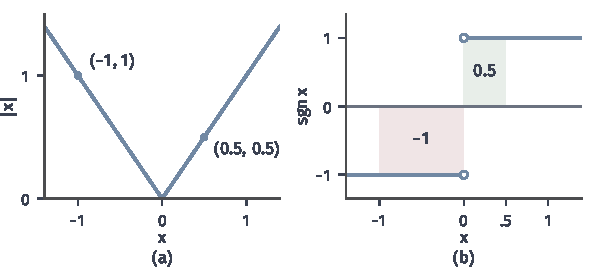
\includegraphics[width=100mm]{figures/04-spaces-measures-and-geometry/02-measure/matplotlib/weakd-abs-sign/figure.pdf}
  \caption{尖点函数与它的弱导数。(a)~$f(x)=\lvert x\rvert$在原点连续但有尖点，两个圆点在一维恢复公式中使用。(b)~弱导数$\operatorname{sgn}x$在原点两侧分别为$-1$与$1$，空心点表示原点的取值可以任意约定，弱导数作为等价类不受影响。填充部分是$[-1,0.5]$上的有向面积，红色部分为$-1$，绿色部分为$0.5$。}
  \label{fig:weakd-abs-sign}
\end{BookInlineFigure}

原点处的两个端点项相消，靠的是$\lvert x\rvert$在原点连续，两侧的极限值相同。下面的阶跃函数在原点断开，同样的计算会在原点留下一项。

\paragraph{跳跃}
取$H=\mathbf 1_{(0,\infty)}$。对测试函数$\varphi$，
\begin{equation}
-\int_{-\infty}^{\infty}H\,\varphi'\,\mathrm dx=-\int_0^\infty\varphi'\,\mathrm dx=\varphi(0).
\label{eq:weakd-step-derivative}
\end{equation}
用上面的$\varphi$可以核对：$\varphi(0)=1$，而
\[
-\int_0^1\varphi'\,\mathrm dx=\varphi(0)-\varphi(1)=1 .
\]

若$H$有弱导数$g$，就应有$\int g\varphi=\varphi(0)$对所有测试函数成立。$H$在原点以外处处可导且经典导数为零，但零函数不满足这个要求：$\int0\cdot\varphi=0$，而$\varphi(0)$可以不为零。不仅零函数不行，任何局部可积函数都不行。

\begin{example}[跳跃不产生局部可积的弱导数]
\label{ex:weakd-step-no-weak-derivative}
反设$g\in L^1_{\mathrm{loc}}(\mathbb R)$使$\int g\varphi=\varphi(0)$对所有测试函数成立。取测试函数
\[
\chi=\mathrm e\,\psi ,
\]
其中$\psi$为式~\eqref{eq:weakd-bump}的隆起函数，$\mathrm e$是自然常数。于是$0\leq\chi\leq1$，$\chi(0)=1$，支撑在$[-1,1]$内。对$0<\varepsilon\leq1$令$\varphi_\varepsilon(x)=\chi(x/\varepsilon)$，它支撑在$[-\varepsilon,\varepsilon]$内，$\varphi_\varepsilon(0)=1$，于是
\[
1=\varphi_\varepsilon(0)=\int g\,\varphi_\varepsilon\,\mathrm dx\leq\int_{-\varepsilon}^{\varepsilon}\lvert g\rvert\,\mathrm dx .
\]
当$\varepsilon\to0$时，$\lvert g\rvert\mathbf 1_{[-\varepsilon,\varepsilon]}$在原点以外逐点趋于零，并被可积函数$\lvert g\rvert\mathbf 1_{[-1,1]}$控制，由支配收敛定理右端趋于零，与左端的$1$矛盾。
\end{example}

例子的机制在图~\ref{fig:weakd-step-spike}(b)中：测试函数的支撑缩到原点时，读数始终是$\varphi_\varepsilon(0)=1$，而任何局部可积函数$g$的积分读数都要乘上越来越短的区间，即使$g$在原点无界，阴影面积也趋于零。跳跃把$H$的全部变化集中在一个点上，这种集中质量正是第~\ref{chap:measure}章中位于原点的单位点质量$\delta_0$。

磨光也说明了同一件事。一维时$H_\varepsilon(x)=\int_{-\infty}^x\rho_\varepsilon$，所以$H_\varepsilon'=\rho_\varepsilon$。图~\ref{fig:weakd-step-spike}(a)中这些导数越来越高越来越窄，面积保持为$1$，极限不是一个函数，而是原点上的集中质量。

\begin{BookInlineFigure}
  \centering
  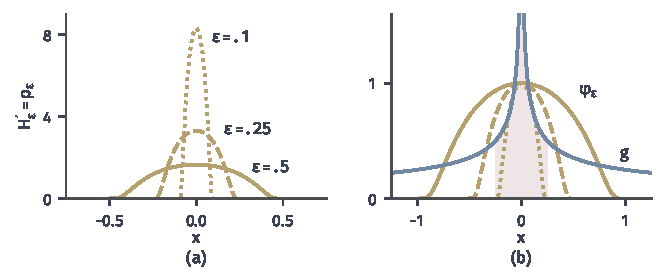
\includegraphics[width=112mm]{figures/04-spaces-measures-and-geometry/02-measure/matplotlib/weakd-step-spike/figure.pdf}
  \caption{跳跃产生集中质量。(a)~磨光后的阶跃函数的导数$H_\varepsilon'=\rho_\varepsilon$，$\varepsilon=0.5,0.25,0.1$，面积都是$1$。(b)~黄色的测试函数$\varphi_\varepsilon$，$\varepsilon=1,0.5,0.25$，在原点的值都是$1$；蓝色是局部可积函数$g(x)=0.25\lvert x\rvert^{-1/2}$，红色阴影是$\varepsilon=0.25$时的积分范围$[-\varepsilon,\varepsilon]$，随$\varepsilon\to0$面积趋于零。}
  \label{fig:weakd-step-spike}
\end{BookInlineFigure}

顺带可知，$\lvert x\rvert$没有二阶弱导数。对测试函数$\varphi$，用上一段的结果和$\operatorname{sgn}x=2H-1$，得到
\[
\int\lvert x\rvert\,\varphi''\,\mathrm dx=-\int\operatorname{sgn}(x)\,\varphi'\,\mathrm dx=2\varphi(0).
\]
要有局部可积的$g$使其等于$\int g\varphi$，同样会与上面的例子矛盾。

\paragraph{分布导数}
两个例子都可以用同一种对象描述。对任意$f\in L^1_{\mathrm{loc}}(\Omega)$与多重指标$\alpha$，规则
\begin{equation}
\varphi\longmapsto(-1)^{\lvert\alpha\rvert}\int_\Omega f\,\partial^\alpha\varphi\,\mathrm dx ,\qquad\varphi\in C_c^\infty(\Omega),
\label{eq:weakd-distributional-derivative}
\end{equation}
把每个测试函数送到一个数，并且对$\varphi$是线性的。由于$\partial^\alpha\varphi$仍是测试函数，式~\eqref{eq:weakd-local-pairing}保证这个数总是有限的。我们把这条线性规则称为$f$的$\alpha$阶\term{分布导数}（distributional derivative）。

有限维的类比是：一个线性泛函总可以写成与某个向量的内积，于是“泛函”和“向量”几乎不用区分。这里的情形不同。分布导数对每个局部可积函数都存在，但这条规则未必能写成与某个局部可积函数的积分；能写成时，那个函数就是弱导数。表~\ref{tab:weakd-distribution-examples}列出前面的例子。

\begin{BookInlineTable}
  \centering
  \begin{tabular}{@{}lll@{}}
    \toprule
    函数 & 分布导数（规则） & 弱导数\\
    \midrule
    $\lvert x\rvert$ & $\varphi\mapsto\int\operatorname{sgn}(x)\,\varphi\,\mathrm dx$ & $\operatorname{sgn}x$\\
    $\operatorname{sgn}x$ & $\varphi\mapsto2\varphi(0)$ & 不存在\\
    $H$ & $\varphi\mapsto\varphi(0)$ & 不存在\\
    \bottomrule
  \end{tabular}
  \caption{一阶分布导数与弱导数。}
  \label{tab:weakd-distribution-examples}
\end{BookInlineTable}

由测试函数判别，能这样表示时$g$几乎处处唯一，所以弱导数就是“能由局部可积函数表示的分布导数”。这类线性规则本身是广义函数理论的研究对象，点质量、读取导数值的规则$\varphi\mapsto-\varphi'(0)$都属于其中；本章只在式~\eqref{eq:weakd-distributional-derivative}的意义下使用分布导数，用它说明弱导数在什么时候不存在。

\subsection{一维弱导数与绝对连续性}
\label{sec:weakd-one-dimension}

$\lvert x\rvert$与阶跃函数的差别还有另一种说法：$\lvert x\rvert$可以由它的导数积分恢复。在图~\ref{fig:weakd-abs-sign}中取两点$x=-1$，$y=0.5$，算出两边：
\[
\lvert y\rvert-\lvert x\rvert=0.5-1=-0.5,\qquad
\int_{-1}^{0.5}\operatorname{sgn}t\,\mathrm dt=-1+0.5=-0.5 .
\]
阶跃函数的经典导数几乎处处为零，积分恒为零，恢复不了原点的跳跃。

第~\ref{chap:integration}章已经证明，有界闭区间上能由可积导数积分恢复的函数恰好是绝对连续函数。本小节证明，在一维情形，“有可积的弱导数”与“有绝对连续代表”是同一件事。下面在有界开区间$(a,b)$上工作，先处理最简单的情形：弱导数为零的函数。

\begin{lemma}[弱导数为零的函数]
\label{lem:weakd-zero-derivative}
设$f\in L^1_{\mathrm{loc}}(a,b)$，且$\int_a^bf\varphi'\,\mathrm dx=0$对所有$\varphi\in C_c^\infty(a,b)$成立。则存在常数$c$，使$f=c$几乎处处。
\end{lemma}

\begin{proof}
先看哪些测试函数是另一个测试函数的导数。设$\psi\in C_c^\infty(a,b)$且$\int_a^b\psi=0$，令
\[
\varphi(x)=\int_a^x\psi(t)\,\mathrm dt .
\]
$\varphi$光滑，$\varphi'=\psi$。在$\operatorname{supp}\psi$左侧$\varphi=0$，在其右侧$\varphi=\int_a^b\psi=0$，所以$\varphi$的支撑在$\operatorname{supp}\psi$的凸包内，是$(a,b)$中的紧集，$\varphi\in C_c^\infty(a,b)$。于是假设给出：$f$与每个积分为零的测试函数相乘后积分为零。

固定一个积分为$1$的测试函数$\theta$，例如中心在区间中点、半径足够小的磨光核。任意测试函数$\psi$可以分解为
\[
\psi=\Bigl(\int_a^b\psi\,\mathrm dx\Bigr)\theta+\Bigl(\psi-\Bigl(\int_a^b\psi\,\mathrm dx\Bigr)\theta\Bigr),
\]
其中第二项积分为零，与$f$相乘后积分为零。

令$c=\int_a^bf\theta\,\mathrm dx$，于是
\[
\int_a^bf\psi\,\mathrm dx=c\int_a^b\psi\,\mathrm dx ,
\]
即$f-c$与所有测试函数相乘后积分为零。由定理~\ref{thm:weakd-test-criterion}，$f=c$几乎处处。
\end{proof}

证明的第一步抓住了一维的特点：积分为零正是一个测试函数能写成另一个测试函数导数的条件。图~\ref{fig:weakd-primitive}比较了两种情形：积分为零时，原函数回到零，支撑仍紧；积分不为零时，原函数停留在一个正的高度，不再是紧支撑的。所以约束$\int f\varphi'=0$只漏掉了一个方向，弱导数为零的函数只剩下一个自由度，即常数。

\begin{BookInlineFigure}
  \centering
  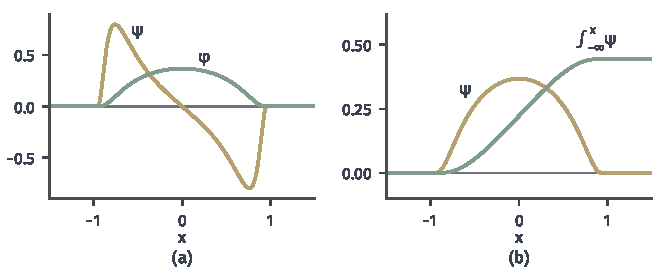
\includegraphics[width=112mm]{figures/04-spaces-measures-and-geometry/02-measure/matplotlib/weakd-primitive/figure.pdf}
  \caption{紧支撑函数的原函数。黄色为$\psi$，绿色为从左端点算起的原函数。(a)~$\psi=\varphi'$的积分为零，原函数$\varphi$回到零，支撑仍在$[-1,1]$内。(b)~$\psi$是隆起函数，积分为$c_1\approx0.444$，原函数在$x\geq1$时停留在$c_1$，不是紧支撑的。}
  \label{fig:weakd-primitive}
\end{BookInlineFigure}

有了这个引理，就可以证明一维的等价定理。

\begin{theorem}[一维弱导数与绝对连续代表]
\label{thm:weakd-absolute-continuity}
设$f,g\in L^1(a,b)$。则$g$是$f$在$(a,b)$上的弱导数，当且仅当存在$[a,b]$上的绝对连续函数$\tilde f$，满足$\tilde f=f$在$(a,b)$上几乎处处成立，并且
\begin{equation}
\tilde f(y)-\tilde f(x)=\int_x^yg(t)\,\mathrm dt ,\qquad a\leq x\leq y\leq b .
\label{eq:weakd-integral-representation}
\end{equation}
这样的$\tilde f$唯一，并且其经典导数$\tilde f'=g$几乎处处成立。
\end{theorem}

\begin{proof}
先说明变上限积分$G(x)=\int_a^xg(t)\,\mathrm dt$以$g$为弱导数。对测试函数$\varphi$，把$G$写成$\int_a^b\mathbf 1_{\{t<x\}}g(t)\,\mathrm dt$，交换积分次序，得到
\[
\begin{aligned}
\int_a^bG\,\varphi'\,\mathrm dx&=\int_a^b\!\!\int_a^b\mathbf 1_{\{t<x\}}\,g(t)\,\varphi'(x)\,\mathrm dt\,\mathrm dx\\
&=\int_a^bg(t)\Bigl(\int_t^b\varphi'(x)\,\mathrm dx\Bigr)\mathrm dt\\
&=-\int_a^bg\,\varphi\,\mathrm dt .
\end{aligned}
\]
交换次序的依据是Fubini定理：$\varphi'$有界，被积函数被$\lvert g(t)\rvert$的常数倍控制，在正方形$[a,b]^2$上可积。最后一步用了$\varphi(b)=0$。

必要性。设$g$是$f$的弱导数，则$f-G$的弱导数为零，由引理~\ref{lem:weakd-zero-derivative}，存在常数$c$使$f=c+G$几乎处处。令$\tilde f=c+G$。由第~\ref{chap:integration}章的微积分基本定理（复值时分实部、虚部），$\tilde f$在$[a,b]$上绝对连续，$\tilde f'=g$几乎处处成立，并满足式~\eqref{eq:weakd-integral-representation}。

充分性。若有满足式~\eqref{eq:weakd-integral-representation}的$\tilde f$，取$x=a$得$\tilde f=\tilde f(a)+G$。常数的弱导数为零，所以$\tilde f$以$g$为弱导数，$f=\tilde f$几乎处处，式~\eqref{eq:weakd-weak-derivative}的两边不变。

唯一性：两个连续函数若几乎处处相等，则在每点相等，因为不相等的点构成开集，而非空开区间的测度为正。
\end{proof}

定理中的端点值属于选定的代表。$f$作为几乎处处等价类没有“在$a$处的值”；正是弱导数的存在，在等价类中选出了唯一一个连续成员$\tilde f$，它在闭区间$[a,b]$上处处有值，包括两个端点。在高维情形，函数及其全部一阶弱导数可积并不保证存在连续代表，这是第~\ref{chap:sobolev-spaces}章嵌入定理研究的问题。

若只假设$f,g\in L^1_{\mathrm{loc}}(a,b)$，结论变为局部的。对每个紧区间$[c,d]\subset(a,b)$，$(c,d)$上的测试函数补零后是$(a,b)$上的测试函数，所以$g$仍是$f$在$(c,d)$上的弱导数，把定理用于$(c,d)$，得到$[c,d]$上的绝对连续代表。这些代表在区间重叠处一致，拼起来是$(a,b)$上的连续函数，在每个紧子区间上绝对连续，却未必能连续延拓到端点。

例如$(0,1)$上$f(x)=\ln x$，弱导数$1/x$局部可积而不可积，$f$在$0$附近无界。局部结论只在内部紧区间上提供积分表示，覆盖整个闭区间的结论需要$f,g$在$(a,b)$上可积。

\begin{example}[有弱导数的无界导数]
\label{ex:weakd-power}
在$(0,1)$上取$f(x)=x^{1/2}$。它是下面这个变上限积分：
\[
f(x)=\int_0^x\tfrac12\,t^{-1/2}\,\mathrm dt .
\]
被积函数可积，
\[
\int_0^1\tfrac12\,t^{-1/2}\,\mathrm dt=1 .
\]
由定理~\ref{thm:weakd-absolute-continuity}，$f$在$[0,1]$上绝对连续，弱导数是$\tfrac12x^{-1/2}$，虽然它在$0$附近无界。阶跃函数则没有绝对连续代表：在$(-1,1)$上，若$H=\mathbf 1_{(0,1)}$有连续代表，它在$(-1,0)$上恒为$0$、在$(0,1)$上恒为$1$，在原点就不可能连续，与上一小节的结论一致。
\end{example}

\subsection{磨光的求导规则}
\label{sec:weakd-mollification-derivative}

图~\ref{fig:weakd-mollifier}中，磨光后的$\lvert x\rvert$的经典导数，看上去恰好是磨光后的$\operatorname{sgn}x$。对有弱导数的函数，这个现象是一般的：先磨光再求经典导数，与先取弱导数再磨光，得到同一个函数。

\begin{theorem}[磨光与弱导数交换]
\label{thm:weakd-mollification-commute}
设$f\in L^1_{\mathrm{loc}}(\Omega)$有弱导数$\partial^\alpha f\in L^1_{\mathrm{loc}}(\Omega)$，$\varepsilon>0$。则在$\Omega_\varepsilon$上
\begin{equation}
\partial^\alpha(f_\varepsilon)=(\partial^\alpha f)_\varepsilon ,
\label{eq:weakd-mollification-commute}
\end{equation}
左端是光滑函数$f_\varepsilon$的经典导数，右端是弱导数的磨光。
\end{theorem}

\begin{proof}
固定$x\in\Omega_\varepsilon$。函数$\varphi_x(y)=\rho_\varepsilon(x-y)$是$\Omega$上的测试函数，定理~\ref{thm:weakd-test-criterion}的证明已核对其支撑。对$y$求导时，链式法则对每个坐标产生一个因子$-1$，所以
\[
\partial_y^\alpha\varphi_x(y)=(-1)^{\lvert\alpha\rvert}(\partial^\alpha\rho_\varepsilon)(x-y).
\]

由定理~\ref{thm:weakd-mollification-smooth}的式~\eqref{eq:weakd-mollifier-derivative}与上式，得到
\[
\begin{aligned}
\partial^\alpha f_\varepsilon(x)&=\int_\Omega(\partial^\alpha\rho_\varepsilon)(x-y)\,f(y)\,\mathrm dy\\
&=(-1)^{\lvert\alpha\rvert}\int_\Omega f\,\partial^\alpha\varphi_x\,\mathrm dy\\
&=\int_\Omega(\partial^\alpha f)\,\varphi_x\,\mathrm dy=(\partial^\alpha f)_\varepsilon(x),
\end{aligned}
\]
第三个等号是弱导数的定义~\eqref{eq:weakd-weak-derivative}用于测试函数$\varphi_x$。
\end{proof}

证明只用了一次弱导数的定义，测试函数恰好是平移、反射后的磨光核。定义中“对所有测试函数成立”的要求在这里被具体地用上了：每个$x$都需要一个不同的测试函数。

\paragraph{函数与导数的同时逼近}
把交换规则与上一节的局部逼近结合，磨光就能在每个内部紧集上同时逼近函数和它的弱导数。

\begin{theorem}[磨光的同时局部逼近]
\label{thm:weakd-simultaneous-approximation}
设$f\in L^1_{\mathrm{loc}}(\Omega)$，$A$是一组有限多个多重指标，对每个$\alpha\in A$，$f$都有弱导数$\partial^\alpha f\in L^1_{\mathrm{loc}}(\Omega)$。设$K\subset\Omega$紧。则$f_\varepsilon$在$K$的一个邻域上光滑，并且当$\varepsilon\to0$时
\begin{equation}
\begin{gathered}
\int_K\lvert f_\varepsilon-f\rvert\,\mathrm dx\to0,\\
\int_K\lvert\partial^\alpha f_\varepsilon-\partial^\alpha f\rvert\,\mathrm dx\to0\quad(\alpha\in A).
\end{gathered}
\label{eq:weakd-simultaneous-approximation}
\end{equation}
\end{theorem}

\begin{proof}
当$\varepsilon<\operatorname{dist}(K,\Omega^{c})$时$K\subset\Omega_\varepsilon$，由定理~\ref{thm:weakd-mollification-smooth}，$f_\varepsilon$在开集$\Omega_\varepsilon$上光滑。第一个极限是定理~\ref{thm:weakd-local-approximation}。

对$\alpha\in A$，由式~\eqref{eq:weakd-mollification-commute}，在$K$上
\[
\partial^\alpha f_\varepsilon-\partial^\alpha f=(\partial^\alpha f)_\varepsilon-\partial^\alpha f .
\]
把定理~\ref{thm:weakd-local-approximation}用于局部可积函数$\partial^\alpha f$即得。$A$有限，所有分量可以同时取充分小的$\varepsilon$。
\end{proof}

以$\lvert x\rvert$为例把两种误差算出来，取$\Omega=\mathbb R$，$K=[-1,1]$，$\varepsilon\leq0.5$。先看导数的误差。由$\operatorname{sgn}x=2H-1$和例~\ref{ex:weakd-step-mollification}的计算，
\[
\int_K\bigl\lvert(\operatorname{sgn})_\varepsilon-\operatorname{sgn}\bigr\rvert\,\mathrm dx=2\varepsilon m_1 .
\]

再看函数本身的误差。记$f(x)=\lvert x\rvert$。把$\rho_\varepsilon$的偶性用上，$A=f_\varepsilon-f$可以写成
\[
A(x)=\int_{\lvert z\rvert\leq\varepsilon}\rho_\varepsilon(z)\,\frac{\lvert x-z\rvert+\lvert x+z\rvert-2\lvert x\rvert}{2}\,\mathrm dz .
\]
由三角不等式，被积函数非负，所以$A\geq0$。

因此误差的积分就是$A$的积分。交换积分次序，并用
\[
\int_{-1}^1\bigl(\lvert x-z\rvert-\lvert x\rvert\bigr)\,\mathrm dx=z^2\qquad(\lvert z\rvert\leq1),
\]
再用替换$z=\varepsilon u$，得到
\[
\int_K\lvert f_\varepsilon-f\rvert\,\mathrm dx=\int_{\lvert z\rvert\leq\varepsilon}\rho_\varepsilon(z)\,z^2\,\mathrm dz=\varepsilon^2m_2 .
\]

表~\ref{tab:weakd-simultaneous-errors}是这两个公式的数值。函数误差按$\varepsilon^2$减小，导数误差按$\varepsilon$减小：弱导数在原点有跳跃，比函数本身更难逼近。

\begin{BookInlineTable}
  \centering
  \begin{tabular}{@{}lll@{}}
    \toprule
    $\varepsilon$ & 函数误差$\varepsilon^2m_2$ & 导数误差$2\varepsilon m_1$\\
    \midrule
    $0.5$ & $0.0395$ & $0.3345$\\
    $0.25$ & $0.0099$ & $0.1672$\\
    $0.1$ & $0.0016$ & $0.0669$\\
    \bottomrule
  \end{tabular}
  \caption{$\lvert x\rvert$的同时逼近误差，$K=[-1,1]$，$m_1\approx0.3345$，$m_2\approx0.1581$。}
  \label{tab:weakd-simultaneous-errors}
\end{BookInlineTable}

阶跃函数$H$的情形不同。$H_\varepsilon$也是光滑函数，它的导数$H_\varepsilon'=\rho_\varepsilon$却不在积分意义下收敛：对任意$\delta>0$，只要$\varepsilon<\delta$，$\rho_\varepsilon$在$\lvert x\rvert\geq\delta$上恒为零，所以极限若是某个函数，只能是零函数；而$\int\rho_\varepsilon=1$并不趋于零。这与$H$没有弱导数相符。

定理~\ref{thm:weakd-simultaneous-approximation}给出的是局部的积分逼近：逼近函数只在离边界大于$\varepsilon$的地方有定义，误差用积分衡量。把这些局部逼近拼成整个区域上的光滑逼近，并在$L^p$范数下控制函数与弱导数的误差，是第~\ref{chap:sobolev-spaces}章光滑稠密性定理的任务。
